% !TeX root = ./0-Tesis-de-maestria-JLBG.tex
\label{cap: teoria metodos}
En este capítulo se emplea el enfoque de la electrodinámica clásica para describir la interacción de un electrón rápido y una nanopartícula (NP) esférica. En particular, se analiza la transferencia de momento angular (TMA) del electrón a la NP. En un trabajo previo de García de Abajo \cite{deabajo2021optical} justifica que, bajo las condiciones descritas en la \hyperref[cap: introduccion]{Introducción}, no es necesaria una descripción cuántica del fenómeno.

Durante el desarrollo matemático, se presentarán las ecuaciones en el Sistema Internacional (SI) en color \textbf{negro}, y en $\cgs{\text{magenta y entre paréntesis}}$\footnote{Se utiliza el \textbf{sistema Internacional} para expresar las ecuaciones en su forma estándar de libro de texto. Sin embargo, las expresiones en el sistema $\cgs{\text{cgs}}$ resultan ideales para realizar una descripción numérica del problema, lo cual se propone como trabajo a futuro. } el factor necesario para expresar la ecuación en el sistema cgs. Por ejemplo, la fuerza entre dos cargas puntuales $q_1$ y $q_2$ separadas una distancia $r$ se escribirá como
\begin{equation}
\vv{F} = \cgs{4\pi\epsilon_0}\frac{1}{4\pi\epsilon_0} \frac{q_1 q_2}{r^2} \hat{r}.
\end{equation}
%
%
\section{Conservación del momento angular en electrodinámica}
Las ecuaciones de Maxwell son \cite{jackson}
%%%%%%%%%%%%%%%% ECUACIONES DE MAXWELL
\begin{align}
\nabla\cdot\vv{E} =& \cgs{4\pi\epsilon_0}\frac{\rho_{\text{tot}}}{\epsilon_0}, \qquad \qquad \nabla\times\vv{E}=-\cgs{\frac{1}{c}}\frac{\partial\vv{B}}{\partial t}, \nonumber \\
\nabla\cdot\vv{B} =& 0, \qquad \qquad \qquad \qquad \nabla\times\vv{B}=\cgs{\frac{4\pi}{\mu_0 c}}\mu_0\vv{J}_{\text{tot}}+\cgs{c}\frac{1}{c^2}\frac{\partial\vv{E}}{\partial t},
\label{eq: Maxwell equations}
\end{align}
dende $\vv{E}$ es el campo eléctrico, $\vv{B}$ es el campo magnético, $\rho_{\rm tot}$ la densidad de carga total, $\vv{J}_{\rm tot}$ es la densidad de corriente total, $c$ es la rapidez de la luz, $\epsilon_0$ es la permitivadad del vacío y $\mu_0$ es la permeabilidad del vacío. Pueden ser reescritas en términos de los potenciales $\phi$ y $\vv{A}$ como \cite{jackson}
%%%%%%%%%%%%%%% ECUACIONES DE ONDA PARA LOS POTENCIALES
\begin{align}
\var{\nabla^2 -\frac{1}{c^2}\frac{\partial}{\partial t}}\phi\vars =& - \cgs{4\pi\epsilon_0} \frac{\rho_{\text{tot}}\vars}{\epsilon_0}, \label{eq: scalar potential}\\
\var{\nabla^2 -\frac{1}{c^2}\frac{\partial}{\partial t}}\vv{A}\vars =& - \cgs{\frac{4\pi}{\mu_0 c}}\mu_0 \vv{J}_{\text{tot}}\vars.\label{eq: vector potential}
\end{align}
Durante el desarrollo teórico se utilizará la norma de Lorentz,  $\nabla\cdot\vv{A}+\cgs{1/c}\partial_t \phi =0$, de modo que los campos electromagnéticos, en términos de los potenciales, se escriben como
%%%%%%%%%%%%%%% ECUACIONES DE CAMPO EN TÉRMINOS DE LOS POTENCIALES
\begin{align}
\vv{E}\vars =& \, -\nabla\phi\vars - \cgs{\frac{1}{c}}\frac{\partial}{\partial t}\vv{A}\vars, \label{eq: E field potentials}\\
\vv{B}\vars =& \, \nabla\times\vv{A}\vars. \label{eq: B field potentials}
\end{align}
La expresión para la conservación del momento lineal en electrodinámica es \cite{jackson}
%%%%%%%%%%%%%%% CONSERVACIÓN DEL MOMENTO LINEAL EN ELECTRODINÁMICA
\begin{equation}
\frac{\partial}{\partial t} \Var{\vv{p}^{\rm \, mec}\var{\vv{r},t}+\vv{p}^{\rm \, em}\var{\vv{r},t}} = \nabla \cdot \tensa{T}\var{\vv{r},t},
\label{eq: cons momento lineal}
\end{equation}
donde $\vv{p}^{\rm \, mec}\var{\vv{r},t}$ es la densidad volumétrica de momento lineal mecánico, $\vv{p}^{\rm \, em}\var{\vv{r},t}$ es la densidad volumétrica de momento lineal electromagnético
%%%%%%%%%%%%%%% MOMENTO LINEAL ELECTROMAGNÉTICO
\begin{equation}
\vv{p}^{\rm \, em}\vars = \cgs{\frac{c}{4\pi}}\frac{1}{c^2}\vv{E}\vars\times\vv{B}\vars
\end{equation}
y $\tensa{T}\var{\vv{r},t}$ es el tensor de esfuerzos de Maxwell dado por \cite{jackson}
%%%%%%%%%%%%%%% TENSOR DE ESFUERZOS DE MAXWELL
\begin{equation}
T_{ij}\var{\vv{r},t}= \frac{\epsilon_0}{\cgs{4\pi\epsilon_0}} \Var{E_i\var{\vv{r},t}E_j\var{\vv{r},t} -\frac{\delta_{ij}}{2}E^2\vars} +  \frac{\mu_0}{\cgs{4\pi\mu_0}} \Var{ H_i\var{\vv{r},t}H_j\var{\vv{r},t} -\frac{\delta_{ij}}{2}H^2\vars } ,
\end{equation}
donde $T_{ij}\var{\vv{r},t}$ es la entrada $ij$ de $\tensa{T}\var{\vv{r},t}$, $E_i\var{\vv{r},t}$ es la $i$-ésima componente del campo eléctrico $\vv{E}\var{\vv{r},t}$, $H_i\var{\vv{r},t}$ es la $i$-ésima componente del campo $\vv{H}\var{\vv{r},t}$ y $\delta_{ij}$ es la delta de Kronecker. 

De la Ec. \eqref{eq: cons momento lineal} se puede deducir la conservación de momento angular en electrodinámica de la siguiente manera
\begin{equation}
\frac{\partial}{\partial t} \Var{\vvb{\ell}^{\rm \, \,mec}\var{\vv{r},t}+\vvb{\ell}^{\rm \, \,em}\var{\vv{r},t}} = \vv{r}\times\nabla \cdot \tensa{T}\var{\vv{r},t},
\label{Eq: r cross P}
\end{equation}
donde $\vvb{\ell}^{\rm \, \,mec}=\vv{r}\times\vv{p}^{\rm \,mec}$ y $\vvb{\ell}^{\rm \, \,em}=\vv{r}\times\vv{p}^{\rm \,em}$ son las densidades volumétricas de momento angular mecánico y electromagnético respectivamente.

Si se define el tensor $\tensa{M}\var{\vv{r},t}=\vv{r}\times\tensa{T}\var{\vv{r},t}$ \textemdash o usando notación de índices y convención de suma de Einstein $M_{jk}\var{\vv{r},t}=\epsilon_{j}^{\,\,\,\, li} r_l T_{ik}\var{\vv{r},t}$\textemdash \,y se calcula la divergencia de $\tensa{M}$, se obtiene 
\begin{align}
\var{\nabla\cdot\tensa{M}}_{j} =& \,\delta^{nk} \partial_n M_{jk} = \delta^{nk} \partial_n \epsilon_{j}^{\,\,\,\, li} r_l T_{ik} =\delta^{nk}\epsilon_{j}^{\,\,\,\, li}\partial_n r_l T_{ik}, \nonumber \\
								=& \,\delta^{nk}\epsilon_{j}^{\,\,\,\, li}\var{\delta_{nl} T_{ik} + r_l \partial_n T_{ik}} =\delta^{nk}\epsilon_{j}^{\,\,\,\, li}r_l\partial_n T_{ik}, \nonumber \\
								=& \,\delta^{nk} \epsilon_{j}^{\,\,\,\, li} r_l \partial_n T_{ik} = \epsilon_{j}^{\,\,\,\, li} r_l \partial^k T_{ik} = \epsilon_{j}^{\,\,\,\, li} r_l \var{\nabla\cdot\tensa{T}}_i, 
\end{align}
de modo que
\begin{equation}
\var{\nabla\cdot\tensa{M}}_{j} = \var{\vv{r}\times \nabla\cdot\tensa{T}}_j,
\label{Eq: Div M}
\end{equation}
donde se ha identificado que $\delta^{nk}\delta_{nl}\,\epsilon_{j}^{\,\,\,\, li}T_{ik} = \epsilon_{j}^{\,\,\,\, ni}T_{in} = 0$, debido a que el tensor de esfuerzos de Maxwell es simétrico $\var{T_{in}=T_{ni}}$ y el símbolo de Levi-Civita es antisimétirco $\var{\epsilon_{j}^{\,\,\,\, ni}=-\epsilon_{j}^{\,\,\,\, in}}$.

De las Ecs. \eqref{Eq: r cross P} y \eqref{Eq: Div M} se escribe la conservación del momento angular como
%
%-------conservation of angular momentum ----------
\begin{empheq}[box=\mymath]{equation}
\frac{\partial}{\partial t} \var{\vvb{\ell}^{\rm \, \,mec}\var{\vv{r},t}+\vvb{\ell}^{\rm \, \,em}\var{\vv{r},t}} = \nabla \cdot \tensa{M}\var{\vv{r},t},
\label{eq: cons momento angular}
\end{empheq}
%-------------------------------------------------
%
que es una ecuación local. Para escribir la conservación del momento angular de forma global, se integra la Ec. \eqref{eq: cons momento angular} sobre un volumen $V$ delimitado por una superficie $S$ de la siguiente manera
%
\begin{mybox}{\centering  Conservación del momento angular global en electrodinámica clásica}
	\begin{equation}
\frac{d}{dt}\Var{\vv{L}^{\rm mec}\var{t}+\vv{L}^{\rm em}\var{t}} = \oint_S \tensa{M}\var{\vv{r},t} \, \cdot d\vv{S},
\label{eq: cons momento angular global}
	\end{equation}
\end{mybox}	
%
% 
\noindent donde se ha usado el teorema de la divergencia en la última igualdad, y se han definido 
\begin{equation}
\vv{L}^{\rm mec}\var{t} = \int_V \vvb{\ell}^{\, \rm mec}\var{\vv{r},t}\, dV, \qquad\qquad \text{y} \qquad\qquad \vv{L}^{\rm em}\var{t} = \int_V \vvb{\ell}^{\, \rm em}\var{\vv{r},t}\, dV.
\end{equation}
Es importante mencionar que la superficie de integración $S$ contiene a la NP pero no interseca a la trayectoria del electrón, como se muestra en la Fig. \ref{fig: system complete}.

\begin{figure}[h!]
\centering
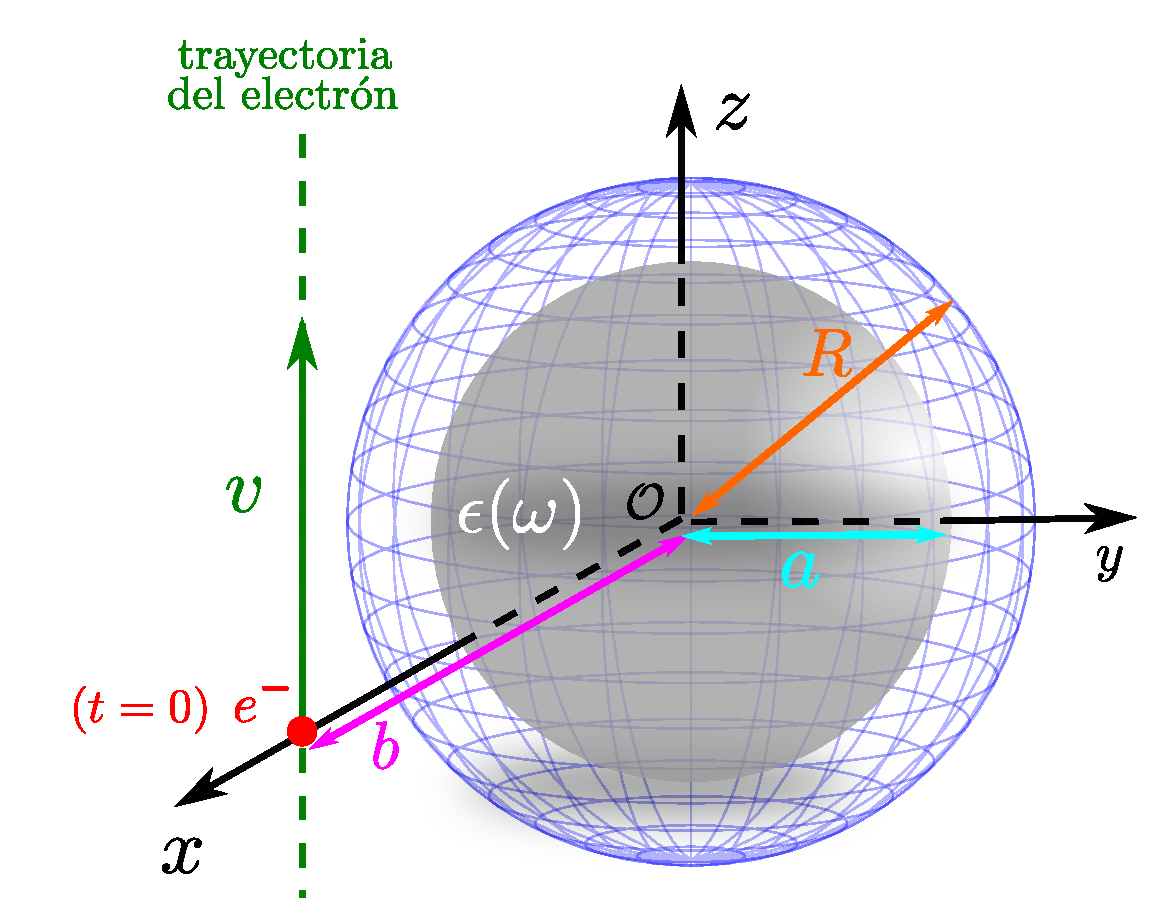
\includegraphics[width=0.5\linewidth]{17-imagenes/2-TeoriaMetodos/system_complete}
\caption{\label{fig: system complete}Nanopartícula centrada en el origen caracterizada por una respuesta dieléctrica homogénea $\epsilon\var{\w}$, encerrada por la superficie de integración $S$ de radio $R$, junto a la trayectoria del electrón colocada en $\vv{r}=(0,b,vt)$.}
\end{figure}

El sistema de estudio consiste en una NP caracterizada por una respuesta dieléctrica homogénea $\epsilon\var{\w}$ centrada en el origen, interactuando con un electrón rápido cuya trayectoria se describe a través de $\vv{r}=(b,0,vt)$, como se muestra en la Fig. \ref{fig: system complete}. Para calcular la transferencia de momento angular (TMA) del electrón a la NP ($\Delta \vv{L}$), se integra la Ec. \eqref{eq: cons momento angular global} a lo largo de toda la trayectoria del electrón, o de manera equivalente en el tiempo de la siguiente manera
\begin{equation}
\Delta\vv{L} = \intt{\frac{d}{dt}\vv{L}^{\rm mec}\var{t}} = \intt{\intS{\tensa{M}\var{\vv{r},t}}} - \Delta\vv{L}^{\rm em},
\end{equation}
donde 
\begin{equation}
\Delta\vv{L}^{\rm em}=\intt{\frac{d}{dt}\vv{L}^{\rm em}} = \vv{L}^{\rm em}(t\to\infty)-\vv{L}^{\rm em}(t\to-\infty).
\end{equation}
El término
\begin{equation}
\vv{L}^{\rm em}(t\to\pm\infty) = \epsilon_0 \mu_0  \intV{\vv{r}\times\Var{\vv{E}\var{t\to\pm\infty}\times\vv{H}\var{t\to\pm\infty}}},
\label{eq: Lem}
\end{equation}
es nulo porque en el tiempo $t\to -\infty$ el electrón se encuentra infinitamente lejos y no ha interactuado con la NP, lo que significa que los campos electromagnéticos totales $\{\EE{},\HH{}\}$, conformados por la suma de los campos externos $\{\EE{ext},\HH{ext}\}$ y esparcidos por la NP $\{\EE{scat},\HH{scat}\}$, son nulos \textemdash$\vv{E}\var{t\to-\infty}=\vv{0}$ y $\vv{H}\var{t\to-\infty}=\vv{0}$\textemdash. Por otro lado, para $t\to\infty$, el electrón se encontrará también infinitamente lejos, pero ya habrá interactuado con la NP, lo que resultará en la inducción de distribuciones de cargas y corrientes eléctricas dentro de la NP. Sin embargo, estas distribuciones habrán desaparecido para $t\to\infty$ debido a procesos disipativos. Por tanto $\vv{L}^{\rm em}\var{t\to\pm\infty}=0$.

Entonces
%
%-------conservation of angular momentum 2----------
\begin{empheq}[box=\mymath]{equation}
\Delta\vv{L} = \intt{\intS{\tensa{M}\var{\vv{r},t}}},
\label{Eq: Delta L in time}
\end{empheq}
%-------------------------------------------------
%
o usando notación de índices
\begin{equation}
\Delta L_i =  \intt{\oint_S \epsilon_{i}^{\,\,\,\, lj} r_l T_{jk}\var{\vv{r},t} n^k\,dS},
\label{eq: angular momentum transfer index notation}
\end{equation}
donde $n_i$ es la $i$-ésima componente del vector normal a la superficie de $S$.

Para el cálculo de la transferencia de momento angular es conveniente expresar los campos electromagnéticos en el espacio de frecuencias. Utilizando la siguiente definición de transformada de Fourier
\begin{equation}
\vv{F}(\w) = \intt{\vv{F}(t)\,{\rm e}^{{\rm i} \w t}} \qquad \text{y} \qquad \vv{F}(t) = \frac{1}{2\pi}\intw{\vv{F}(\w)\,{\rm e}^{-{\rm i} \w t}},
\end{equation}
donde $\vv{F}\in \{ \vv{B}, \vv{H}\}$ y para que $\vv{F}(t)$ sea una función de variable real se debe cumplir en el espacio de frecuencias que $\vv{F}(\w)^{*}=\vv{F}(-\w)$, donde $*$ denota complejo conjugado. Para calcular la TMA a través de la Ec. \eqref{eq: angular momentum transfer index notation} es importante notar que la dependencia en el tiempo está contenida únicamente en el tensor de esfuerzos de Maxwell $\tensa{T}\var{\vv{r},t}$. De esta forma, se puede reescribir la integral en el tiempo del producto de campos eléctricos de la siguiente manera
\begin{align}
\intt{E_i\vars E_j \vars} =& \intt{\Var{\frac{1}{2\pi}\intw{E_i\varsw \,{\rm e}^{-{\rm i} \w t} }} \Var{\frac{1}{2\pi}\intw{E_j\var{\vv{r},\w^{\prime}} \,{\rm e}^{-{\rm i} \w^{\prime} t} }^{\prime}} } \nonumber\\
=&\frac{1}{2\pi} \intw{\intw{\Var{\frac{1}{2\pi}\intt{{\rm e}^{-{\rm i}\var{\w+\w^{\prime}} t}}} E_i \varsw E_j\var{\vv{r},\w^{\prime}}}}^{\prime} \nonumber\\
=&\frac{1}{2\pi}\intw{\intw{\delta\var{\w+\w^{\prime}} E_i \varsw E_j\var{\vv{r},\w^{\prime}} }}^{\prime} \nonumber\\
=&\frac{1}{2\pi}\intw{ E_i \varsw E_j\var{\vv{r},-\w} }=\frac{1}{2\pi}\intw{ E_i \varsw E_j^{*}\varsw } \nonumber\\
=&\frac{1}{\pi}\intwo{{\rm Re}\Var{E_i\varsw E_j^{*}\varsw}}.
\end{align}
Para las componentes del campo $\vv{H}$ se requiere un proceso análogo.

De esta manera se puede reescribir la Ec. \eqref{eq: angular momentum transfer index notation} como
%
%-------Angular momentum transfer----------
\begin{empheq}[box=\mymath]{equation}
\Delta L_i = \frac{1}{\pi} \intwo{\oint_S \epsilon_{i}^{\,\,\,\, lj} r_l \mathcal{T}_{jk}\varsw n^k\,dS},
\label{eq: angular momentum transfer index notation freq domain}
\end{empheq}
%-------------------------------------------------
%
donde se ha definido 
\begin{align}
\tensa{\mathcal{T}}\varsw = \,{\rm Re}\Bigg[&\frac{\epsilon_0}{\cgs{4\pi\epsilon_0}} \vv{E} \varsw \vv{E}^{*}\varsw-\frac{\epsilon_0}{\cgs{4\pi\epsilon_0}} \frac{\tensa{I}}{2} \vv{E} \varsw\cdot\vv{E}_j^{*}\varsw \nonumber \\
& + \frac{\mu_0}{\cgs{4\pi\mu_0}} \vv{H}_i \varsw \vv{H}_j^{*}\varsw- \frac{\mu_0}{\cgs{4\pi\mu_0}} \frac{\tensa{I}}{2}  \vv{H} \varsw\cdot\vv{H}^{*}\vars \Bigg], \label{Eq: tensor maxwell freq}
\end{align}
donde $\tensa{I}$ es el tensor identidad de rango 2. De esta forma se define finalmente la <<densidad espectral>> de momento angular como
%
%-------Spectral density----------
\begin{empheq}[box=\mymath]{equation}
\mathcal{L}_i\var{\w} = \frac{1}{\pi} \oint_S \epsilon_{i}^{\,\,\,\, lj} r_l \mathcal{T}_{jk}\varsw n^k\,dS. \label{Eq: spectral density AMT}
\end{empheq}
%-------------------------------------------------
%
por lo que la TMA se calcula de la siguiente forma
\begin{equation}
\Delta \vv{L} = \intwo{\vv{\mathcal{L}}\var{\w}}.
\label{eq: densidad espectral momento angular}
\end{equation}

En coordenadas cartesianas la Ec. \eqref{Eq: spectral density AMT} puede ser escrita como
\begin{align}
\mathcal{L}_x &=\frac{1}{\pi}\Var{\oint_{S} y\, \mathcal{T}_{zk}\, dS^k - \oint_{S} z\, \mathcal{T}_{yk}\, dS^k },\\
\mathcal{L}_y &=\frac{1}{\pi}\Var{\oint_{S} z\, \mathcal{T}_{xk}\, dS^k - \oint_{S} x\, \mathcal{T}_{zk}\, dS^k },\label{eq: Ly spectral density}\\
\mathcal{L}_z &=\frac{1}{\pi}\Var{\oint_{S} x\, \mathcal{T}_{yk}\, dS^k - \oint_{S} y\, \mathcal{T}_{xk}\, dS^k }. 
\end{align}

Debido a que el problema de interacción de un electrón rápido interactuando con una NP esférica presenta  simetría de reflexión con respecto al plano $xz$, no puede haber componente de momento lineal transferido en la dirección $y$ \cite{PRBCoronado}. De lo anterior se puede concluir que el momento angular transferido a la NP no puede tener componente $x$ ni $z$ \cite{castellanos2021phdthesis}. Por tanto, resulta que solamente la contribución espectral $\mathcal{L}_y$ es diferente de cero. Se puede reescribir la componente espectral en términos de proyecciones esféricas en lugar de cartesianas, de la siguiente manera \cite{castellanos2021phdthesis}
%
\begin{mybox}{\centering  Componente espectral que contribuye a la transferencia de momento angular}
\begin{equation}
\mathcal{L}_y = \frac{1}{\pi}\oint \sin\theta \Var{\cos\varphi \,\mathcal{T}_{\theta r} - \cos\theta\sin\varphi\,\mathcal{T}_{\varphi r}} dS_r,
\label{eq: Ly spectral density r theta}
\end{equation}
\end{mybox}	
% 
y
%
\begin{mybox}{\centering  Componentes espectrales que no contribuyen a la transferencia de momento angular}
\begin{align}
\mathcal{L}_x &= \frac{1}{\pi}\oint \sin\theta \Var{\cos\varphi \,\mathcal{T}_{\theta r} - \cos\theta\sin\varphi\,\mathcal{T}_{\varphi r}} dS_r,
\label{eq: Lx spectral density r theta} \\
\mathcal{L}_x &= \frac{1}{\pi}\oint \sin^2\theta \, \mathcal{T}_{\varphi r} \, dS_r,
\label{eq: Lz spectral density r theta}
\end{align}
\end{mybox}	
% 
\noindent donde se ha asumido una superficie de integración esférica, como se muestra en la Fig. \ref{fig: system complete}.

Dado que los campos $\EE{}$ y $\HH{}$ que aparecen en la Ec. \eqref{Eq: tensor maxwell freq} corresponden a los campos totales, suma del campo producido por el electrón y el esparcido por la NP, es posible separar la contribución eléctrica de la magnética en la densidad espectral de momento angular en la Ec. \eqref{eq: densidad espectral momento angular}, de modo que se puede separar el tensor de la siguiente forma

\begin{equation}
\tensa{\mathcal{T}}\varsw = \tensE{\mathcal{T}}\varsw+\hspace{-0.2 cm}\tensH{\mathcal{T}}\varsw, 
\end{equation}
donde 
\begin{align}
\tensE{\mathcal{T}}=& \frac{\epsilon_0}{\cgs{4\pi\epsilon_0}} \re{\vv{E}\varsw \vv{E}^{*}\varsw - \frac{\tensa{I}}{2} \vv{E}\varsw\cdot\vv{E}^{*}\varsw}
\end{align}
y
\begin{align}
\hspace{0.3 cm}\tensH{\mathcal{T}}=& \frac{\mu_0}{\cgs{4\pi\mu_0}} \re{\vv{H}\varsw \vv{H}^{*}\varsw - \frac{\tensa{I}}{2} \vv{H}\varsw\cdot\vv{H}^{*}\varsw}.
\end{align}

Dado que se está considerando una superficie $s$ de integración esférica de radio $R$ y a $\hat{r}_i$ como la $i$-ésima componente del vector unitario radial, la densidad espectral de momento angular $\mathcal{L}_i(\w)$ se puede escribir como
\begin{equation}
\mathcal{L}_i\var{\w} = \frac{R^2}{\pi} \int_0^{4\pi} \Var{\epsilon_{i}^{\,\,\,\, lj} r_l \mathcal{T}^{\, \rm E}_{jk}\varsw n^k + \epsilon_{i}^{\,\,\,\, lj} r_l \mathcal{T}^{\, \rm H}_{jk}\varsw n^k}\,d\Omega,
\label{Eq: complete spectral component of AMT with spherical symmetry}
\end{equation}
donde únicamente falta integrar en el ángulo sólido $\Omega$. En la Ec. \eqref{Eq: complete spectral component of AMT with spherical symmetry} se observa que la contribución eléctrica está separada de la magnética, de modo que se pueden definir ambas contribuciones como
\begin{align}
\mathcal{L}_i^{\rm E}\var{\w} = \frac{R^2}{\pi} \int_0^{4\pi} \Var{\epsilon_{i}^{\,\,\,\, lj} r_l \mathcal{T}^{\,\rm E}_{jk}\varsw n^k}\,d\Omega, \\
\mathcal{L}_i^{\rm H}\var{\w} = \frac{R^2}{\pi} \int_0^{4\pi} \Var{\epsilon_{i}^{\,\,\,\, lj} r_l \mathcal{T}^{\,\rm H}_{jk}\varsw n^k}\,d\Omega.
\end{align}

Dado que se pueden separar a los campos electromagnéticos $\vv{E}$ y $\vv{H}$ en sus contribuciones de campo externo (ext) y campo esparcido (scat) como 
\begin{equation}
\vv{E} = \EE{ext} + \EE{scat}, \qquad\qquad \text{y} \qquad\qquad \vv{H} = \HH{ext} + \HH{scat},
\end{equation}
donde $\EE{ext}$ y $\HH{ext}$ son los campos electromagnéticos externos \textemdash producidos por el electrón\textemdash, y $\EE{scat}$ y $\HH{scat}$ son los campos esparcidos por la NP. Se reescribe la componente eléctrica del tensor de la Ec. \eqref{Eq: tensor maxwell freq} como
\begin{align}
\tensE{\mathcal{T}}=\,\frac{\epsilon_0}{\cgs{4\pi\epsilon_0}} {\rm Re} \Bigg[& \var{\EE{ext}+\EE{scat}}\var{\EE{ext}^{*}+\EE{scat}^{*}}-\frac{\tensa{I}}{2}\var{\EE{ext}+\EE{scat}}\cdot\var{\EE{ext}^{*}+\EE{scat}^{*}} \Bigg] \nonumber \\
= \, \frac{\epsilon_0}{\cgs{4\pi\epsilon_0}} {\rm Re} \Bigg[& \var{\EE{scat}\EE{scat}^{*}+\EE{scat}\EE{ext}^{*}+\EE{ext}\EE{scat}^{*}+\EE{ext}\EE{ext}^{*}}\nonumber \\
&-\frac{\tensa{I}}{2}\var{\EE{scat}\cdot\EE{scat}^{*}+\EE{scat}\cdot\EE{ext}^{*}+\EE{ext}\cdot\EE{scat}^{*}+\EE{ext}\cdot\EE{ext}^{*}} \Bigg],
\label{eq: tensor de esfuerzos inicio}
\end{align}
donde la componente eléctrica del tensor de esfuerzos se escribe como
\begin{equation}
\tensE{\mathcal{T}}=\tensE{\mathcal{T}}_{\rm ss}+\tensE{\mathcal{T}}_{\rm int}+\tensE{\mathcal{T}}_{\rm ee},
\end{equation}
con
\begin{align}
\tensE{\mathcal{T}}_{\rm ss} =& \frac{\epsilon_0}{\cgs{4\pi\epsilon_0}} \re{\EE{scat}\EE{scat}^{*}-\frac{\tensa{I}}{2}\EE{scat}\cdot\EE{scat}^{*}},\label{Eq: tensor de esfuerzos inicio 2}\\
\tensE{\mathcal{T}}_{\rm ee} =& \frac{\epsilon_0}{\cgs{4\pi\epsilon_0}} \re{\EE{ext}\EE{ext}^{*}-\frac{\tensa{I}}{2}\EE{ext}\cdot\EE{ext}^{*}}, \label{Eq: Tee}\\
&\tensE{\mathcal{T}}_{\rm int} = \tensE{\mathcal{T}}_{\rm se} + \tensE{\mathcal{T}}_{\rm es},
\end{align}
donde
\begin{align}
\tensE{\mathcal{T}}_{\rm es} =& \frac{\epsilon_0}{\cgs{4\pi\epsilon_0}} \re{\EE{ext}\EE{scat}^{*}-\frac{\tensa{I}}{2}\EE{ext}\cdot\EE{scat}^{*}},\label{Eq: Tes}\\
\tensE{\mathcal{T}}_{\rm se} =& \frac{\epsilon_0}{\cgs{4\pi\epsilon_0}} \re{\EE{scat}\EE{ext}^{*}-\frac{\tensa{I}}{2}\EE{scat}\cdot\EE{ext}^{*}}.
\label{eq: tensor de esfuerzos final}
\end{align}
Análogamente, al hacer la sustitución $\epsilon_0 \to \mu_0$ y $\vv{E}\to\vv{H}$ en las Ecs. \eqref{eq: tensor de esfuerzos inicio}-\eqref{eq: tensor de esfuerzos final}, se obtienen las contribuciones magnéticas al tensor $\tensa{\mathcal{T}}$, denotadas por $\hspace{-0.6 em}\tensH{\mathcal{T}}_{\rm ij}$ donde $\rm ij$ toman los valores \{$\rm e$, $\rm s$\}.

Se puede interpretar a $\tensa{\mathcal{T}}_{\rm int}$ como la componente que está relacionada con la interacción del campo electromagnético del electrón con las cargas y corrientes inducidas en la NP. En el caso en que no existiera NP, nada alteraría el movimiento del electrón, por lo que no perdería ni cedería energía, momento lineal ni momento angular ($\Delta L = 0$) \cite{castellanos2021phdthesis}. En este caso los campos electromagnéticos esparcidos serían nulos, por lo que la única contribución al momento angular provendría de la componente $\tensa{\mathcal{T}}_{\rm ee}$. Por tanto, de manera general, se concluye que la contribución al momento angular transferido debido a $\tensa{\mathcal{T}}_{\rm ee}$ es nula. También es conveniente mencionar que la componente $\tensa{\mathcal{T}}_{\rm ss}$, al depender únicamente de los campos electromagnéticos esparcidos por la NP, está relacionada con la interacción de la NP consigo misma, referida por algunos autores como reacción de radiación \cite{jackson}.  

En la siguiente sección se presentan las expresiones analíticas de los campos electromagnéticos externos (producidos por el electrón), así como de los esparcidos por la NP.
%
% 	TRANSFERENCIA DE MOMENTO ANGULAR DE UN ELECTRÓN RÁPIDO A UNA NANOPARTÍCULA ESFÉRICA
%
\section{Transferencia de momento angular de un electrón rápido a una nanopartícula}
El campo electromagnético externo producido por un electrón rápido, considerado como una partícula puntual de carga $q=-e$, viajando a velocidad $\vv{v}$ constante a lo largo del eje z a lo largo de la trayectoria $\vv{r}=(b,0,vt)$ (ver Fig. \ref{fig: system complete}), se puede obtener mediante una transformación de Lorentz de un sistema de referencia en el que el electrón se encuentra en reposo, a un sistema de referencia en el que el electrón que se mueve a velocidad constante $\vv{v}$, obteniendo \cite{jackson}
\begin{align}
\EE{ext}\vars =& \cgs{4\pi\epsilon_0}\frac{-e}{4\pi\epsilon_0}\frac{\gamma \Var{\vv{R}+(z-vt)\hat{z}}}{\Var{R^2+\gamma^2(z-vt)^2}^{3/2}}, \label{eq: Eext}\\
\HH{ext}\vars =& \cgs{4\pi}\frac{-e}{4\pi}\frac{\gamma \, \vv{v}\times\vv{R}}{\Var{R^2+\gamma^2(z-vt)^2}^{3/2}}, \label{eq: Hext}
\end{align}
en donde $c$ es la rapidez de la luz, $\gamma = \var{1-\beta^2}^{-1/2}$, $\beta = v/c$, $\vv{R}=(x-b)\hat{x}+y\hat{y}$, $R = \sqrt{(x-b)^2+y^2}$ y $\vv{v}\times\vv{R}=v\Var{(x-b)\hat{y}-y\hat{x}}$. También se pueden calcular los campos electromagnéticos externos en función de la frecuencia mediante una transformada de Fourier de las Ecs. \eqref{eq: Eext} y \eqref{eq: Hext} \cite{maciel2019electromagnetic}:
%-------E & H fields in freq space----------
\begin{empheq}[box=\mymath]{align}
\EE{ext}\varsw = &\cgs{4\pi\epsilon_0}\frac{-e}{4\pi\epsilon_0}  \frac{2\w}{v^2 \gamma} \rme^{\rmi \w (z/v)} \left\{ {\rm sign}(\w) K_1\wR\hat{R} - \frac{\rmi}{\gamma}K_0\wR \hat{z}\right\},\\
&\HH{ext}\varsw = \cgs{4\pi}\frac{-e}{4\pi}\frac{2e}{v c \gamma} \abs{\omega} {\rm e}^{{\rm i}\omega z /v} K_1\wR \hat{v}\times\hat{R},
\end{empheq}
%-------------------------------------------------
que son expresiones cerradas con simetría cilíndrica. Dado que para el cálculo de la TMA son necesarios los campos esparcidos por la NP, que tienen simetría esférica, conviene expresar a los campos electromagnéticos del electrón mediante una solución con simetría esférica. 

El campo eléctrico producido por el electrón se puede obtener mediante la función de Green dependiente del tiempo \cite{maciel2019electromagnetic}  
\begin{equation}
\EE{ext}\varsw = e\var{\nabla-\rmi \frac{k\vv{v}}{c}} \intt{\rme^{\rmi \w t} G_0 \var{\vv{r}-\vv{r}_t}},
\label{eq: E field Green function}
\end{equation}
donde la función de Green $G_0 \var{\vv{r}-\vv{r}_t}$ está dada por 
\begin{equation}
G_0 \var{\vv{r}-\vv{r}_t} = \frac{\cgs{4\pi\epsilon_0}}{4\pi\epsilon_0}\frac{\rme^{\rmi k \abs{\vv{r}-\vv{r}_t}}}{\abs{\vv{r}-\vv{r}_t}},
\end{equation}
con $k = \w/c$ el número de onda en el vacío, $\vv{r}_t=\vv{r}_0+\vv{v}t$ la posición del electrón al tiempo $t$ y $\vv{r}_0 = (b,0,0)$. Al expandir la función de Green en base esférica se obtiene \cite{de1999relativistic}
\begin{equation}
G_0(\vv{r}-\vv{r}_t) = \frac{\cgs{4\pi\epsilon_0}}{\epsilon_0} k \sum_{\ell = 0}^{\infty} \sum_{m=-\ell}^{\ell} j_{\ell}(kr) h_{\ell}^{+}(k r_t) Y_{\ell, m}(\Omega_r) Y_{\ell, m}(\Omega_{r_t})^{*},
\label{eq: Green function spherical base}
\end{equation}
donde $Y_{\ell,m}$ son los armónicos esféricos escalares, $\Omega_r$ es el ángulo sólido del vector $\vv{r}$, $h_{\ell}^{+}(x) = \rmi h_{\ell}^{1}(x)$ es la función de Hankel esférica de orden $\ell$ y $j_{\ell}(x)$ es la función esférica de Bessel de orden $\ell$ \citep{Abramowitz}. Sustituyendo la Ec. \eqref{eq: Green function spherical base} en la Ec. \eqref{eq: E field Green function}, se obtiene
\begin{equation}
\EE{ext}\vars = \var{\nabla-\rmi \frac{k\vv{v}}{c}} \sum_{\ell = 0}^{\infty} \sum_{m=-\ell}^{\ell} j_{\ell}(kr) Y_{\ell, m}(\Omega_{r})\phi_{\ell, m},
\end{equation}
donde 
\begin{equation}
\phi_{\ell, m} = \frac{\cgs{4\pi\epsilon_0}}{\epsilon_0} k \intt{e^{i \omega t} h_{\ell}^{+}(k r_{t}) Y_{\ell, m}^{*}(\Omega_{r_t}) }.
\label{Eq: GdA phi coeffs}
\end{equation}

En el \hyperref[AppendixScalarPotentials]{Apéndice A} se muestran los detalles del cálculo analítico de la Ec. \eqref{Eq: GdA phi coeffs}. Entonces, el campo electromagnético externo en representación multipolar esférica se escribe como:

%
\begin{mybox}{\centering  Expansión multipolar del campo electromagnético externo producido por el electrón}
\vspace{-0.3cm}
\begin{align}
\EE{ext} &= \sum_{\ell, m} \var{\mathscr{E}_{\ell, m}^{\text{er}}\hat{r} +\mathscr{E}_{\ell, m}^{\text{e}\theta}\hat{\theta} + \mathscr{E}_{\ell, m}^{\text{e}\varphi}\hat{\varphi}},\label{Eq: multipolar ext E field}\\
\HH{ext} &= \sum_{\ell, m} \var{\mathscr{H}_{\ell, m}^{\text{er}}\hat{r} +\mathscr{H}_{\ell, m}^{\text{e}\theta}\hat{\theta} + \mathscr{H}_{\ell, m}^{\text{e}\varphi}\hat{\varphi}},
\end{align}
\end{mybox}	
%
% 
\noindent donde
%
%-------Components of ext electric field ----------
\begin{empheq}[box=\mymath]{align}
& \qquad\qquad \mathscr{E}_{\ell, m}^{\text{er}}=\rme^{\rmi m \varphi} D_{\ell, m}^{\text{ext}} \ell (\ell +1 ) P_{\ell}^{m}\var{\cos\theta}\frac{j_{\ell}\var{k r}}{k r},\label{eq: Elmer}\\
%
\mathscr{E}_{\ell, m}^{\text{e}\theta}=&-\rme^{\rmi m \varphi}C_{\ell, m}^{\text{ext}} \frac{m}{\sin\theta}j_{\ell}\var{k r}P_{\ell}^{m}(\cos\theta)-\rme^{\rmi m \varphi}D_{\ell, m}^{\text{ext}}\bigg[ \var{\ell + 1}\frac{\cos\theta}{\sin\theta} P_{\ell}^{m}\var{\cos\theta}- \nonumber \\
&\frac{\var{\ell-m+1}}{\sin\theta}P_{\ell+1}^{m}\var{\cos\theta} \bigg] \Var{\var{\ell +1}\frac{j_{\ell}\var{k r}}{k r}-j_{\ell +1}\var{k r}}, \label{eq: Elmet}\\
%
\mathscr{E}_{\ell, m}^{\text{e}\varphi}=& \,\rmi\, \rme^{\rmi m \varphi}C_{\ell, m}^{\text{ext}}\, j_{\ell}\var{k r}\Var{\var{\ell +1}\frac{\cos\theta}{\sin\theta}P_{\ell}^{m}\var{\cos\theta}-\frac{\ell-m+1}{\sin\theta}P_{\ell +1}^{m}\var{\cos\theta}} \nonumber \\
&+\rmi\,\rme^{\rmi m \varphi}D_{\ell, m}^{\text{ext}}\frac{m}{\sin\theta}P_{\ell}\var{\cos\theta}\Var{\var{\ell +1}\frac{j_{\ell}\var{k r}}{k r}-j_{\ell + 1}(k r)}, \label{eq: Elmep}
\end{empheq}
%-------------------------------------------------
%
y
%
%-------Components of ext electric field ----------
\begin{empheq}[box=\mymath]{align}
& \qquad\qquad \mathscr{H}_{\ell, m}^{\text{er}}=\rme^{\rmi m \varphi} C_{\ell, m}^{\text{ext}} \ell (\ell +1 ) P_{\ell}^{m}\var{\cos\theta}\frac{j_{\ell}\var{k r}}{k r}, \label{eq: Hlmer}\\
%
\mathscr{H}_{\ell, m}^{\text{e}\theta}=&\,\rme^{\rmi m \varphi}D_{\ell, m}^{\text{ext}} \frac{m}{\sin\theta}j_{\ell}\var{k r}P_{\ell}^{m}(\cos\theta)-\rme^{\rmi m \varphi}C_{\ell, m}^{\text{ext}}\bigg[ \var{\ell + 1}\frac{\cos\theta}{\sin\theta} P_{\ell}^{m}\var{\cos\theta}- \nonumber \\
&\frac{\var{\ell-m+1}}{\sin\theta}P_{\ell+1}^{m}\var{\cos\theta} \bigg] \Var{\var{\ell +1}\frac{j_{\ell}\var{k r}}{k r}-j_{\ell +1}\var{k r}}, \label{eq: Hlmet}\\
%
\mathscr{H}_{\ell, m}^{\text{e}\varphi}=&- \,\rmi\, \rme^{\rmi m \varphi} D_{\ell, m}^{\text{ext}}\, j_{\ell}\var{k r}\Var{\var{\ell +1}\frac{\cos\theta}{\sin\theta}P_{\ell}^{m}\var{\cos\theta}-\frac{\ell-m+1}{\sin\theta}P_{\ell +1}^{m}\var{\cos\theta}} \nonumber \\
&+\rmi\,\rme^{\rmi m \varphi}C_{\ell, m}^{\text{ext}}\frac{m}{\sin\theta}P_{\ell}\var{\cos\theta}\Var{\var{\ell +1}\frac{j_{\ell}\var{k r}}{k r}-j_{\ell + 1}(k r)}, \label{eq: Hlmep}
\end{empheq}
%-------------------------------------------------
%
donde $P_{\ell}^{m}$ son las funciones asociadas de Legendre, y los coeficientes escalares $C_{\ell, m}^{\text{ext}}$ y $D_{\ell, m}^{\text{ext}}$ están dados por
%
%-------Ckm & Dlm ext coeffs ----------
\begin{empheq}[box=\mymath]{align}
C_{\ell, m}^{\text{ext}} =& \rmi^{\ell}\sqrt{\frac{2\ell +1}{4\pi}\frac{\var{\ell - m}!}{\var{\ell +m}!}}\psi_{\ell, m}^{\rm M, \text{ext}}, \label{Eq: C ext l,m} \\
D_{\ell, m}^{\text{ext}} =& \rmi^{\ell}\sqrt{\frac{2\ell +1}{4\pi}\frac{\var{\ell - m}!}{\var{\ell +m}!}}\psi_{\ell, m}^{\rm E, \text{ext}}, \label{Eq: D ext l,m}
\end{empheq} 
%-------------------------------------------------
% 
con $\psi_{\ell, m}^{E, \text{ext}}$ y $\psi_{\ell, m}^{M, \text{ext}}$ los coeficientes de la representación esférica de los potenciales auxiliares, definidos en el \hyperref[AppendixScalarPotentials]{Apéndice A}.
%
\section{Campos electromagnéticos esparcidos por la nanopartícula}
Como se muestra en el \hyperref[AppendixScalarPotentials]{Apéndice A}, los campos electromagnéticos satisfacen la ecuación de Helmholtz sin fuentes
\begin{align}
\var{\nabla^2+k^2}\EE{} = \vv{0},\label{Eq: Helmholtz E}\\
\var{\nabla^2+k^2}\HH{} = \vv{0}.\label{Eq: Helmholtz H}
\end{align}
%donde $k^2 = \cgs{c^{-2}}\w^2\epsilon\var{\w}\mu\var{\w}$. 
La solución de las Ecs. \eqref{Eq: Helmholtz E} y \eqref{Eq: Helmholtz H} puede ser escrita como \cite{Low}
\begin{align}
\EE{} &= \nabla\psi^{\rm L} + \vv{L}\psi^{\rm M}-\frac{\rmi}{k}\nabla\times\vv{L}\psi^{\rm E}, \label{Eq: E field in terms of potentials}\\
\HH{} &= -\frac{\rmi}{k}\nabla\times\vv{L}\psi^{M}-\vv{L}\psi^{\rm E}, \label{Eq: H field in terms of potentials}
\end{align}
donde $\vv{L}=-\rmi \vv{r}\times\nabla$ es el operador de momento angular orbital y $\psi^{\rm L}$, $\psi^{\rm E}$ y $\psi^{\rm M}$ son  funciones escalares que satisfacen la ecuación escalar de Helmholtz. Como el campo eléctrico externo es un campo solenoidal ($\nabla\cdot\EE{}=0$), la función escalar $\psi^{\rm L}$ debe ser nula. Las funciones escalares $\psi^{\rm E}$ y $\psi^{\rm M}$, del campo externo y del campo esparcido, respectivamente, pueden ser expandidas en una base esférica definida a partir del sistema de coordenadas mostrado en la Fig. \ref{fig: system complete}, como \cite{de1999relativistic}
\begin{align}
\psi^{\rm E, \text{ext}}(\vv{r})=\sum_{\ell =1}^{\infty}\sum_{m=-\ell}^{\ell}\rmi^{\ell}j_{\ell}\var{kr}Y_{\ell, m}(\Omega_r)\psi_{\ell, m}^{\rm E, \text{ext}},\\
\psi^{\rm E, \text{ext}}(\vv{r})=\sum_{\ell =1}^{\infty}\sum_{m=-\ell}^{\ell}\rmi^{\ell}j_{\ell}\var{kr}Y_{\ell, m}(\Omega_r)\psi_{\ell, m}^{\rm E, \text{ext}},\\
\psi^{\rm E, \text{scat}}(\vv{r})=\sum_{\ell =1}^{\infty}\sum_{m=-\ell}^{\ell}\rmi^{\ell}h_{\ell}^{+}\var{kr}Y_{\ell, m}(\Omega_r)\psi_{\ell, m}^{\rm E, \text{scat}},\\
\psi^{\rm E, \text{scat}}(\vv{r})=\sum_{\ell =1}^{\infty}\sum_{m=-\ell}^{\ell}\rmi^{\ell}h_{\ell}^{+}\var{kr}Y_{\ell, m}(\Omega_r)\psi_{\ell, m}^{\rm E, \text{scat}}.
\end{align}
Aplicando las condiciones de frontera de los campos electromagnéticos para una partícula esférica, se pueden calcular los potenciales escalares electromagnéticos esparcidos por la NP en función de los potenciales escalares electromagnéticos externos de la siguiente manera \cite{de1999relativistic}
\begin{align}
\psi_{\ell, m}^{\rm E, scat} =& \,t_{\ell}^{\rm E} \psi_{\ell, m}^{\rm E, \text{ext}}, \label{Eq: psilm E scat}\\
\psi_{\ell, m}^{\rm M, scat} =& \,t_{\ell}^{\rm M} \psi_{\ell, m}^{\rm M, \text{ext}}, \label{Eq: psilm M scat}
\end{align} 
donde los coeficientes $t_{\ell}^{\rm E}$ y $t_{\ell}^{\rm M}$, para el caso de partículas esféricas homogéneas, corresponden a los coeficientes de la solución de Mie: \cite{Bohren}

\begin{align}
t_{\ell}^{\rm E} &=\frac{-j_{\ell}(x_0)\Var{x_i j_{\ell}(x_i)}^{\prime}+\epsilon_i\,j_{\ell}(x_i)\Var{x_0j_{\ell}(x_0)}^{\prime}}{h^{+}\var{x_0}\Var{x_i j_l\var{x_i}}^{\prime}-\epsilon_i j_l\var{x_i}\Var{x_0 h_{\ell}^{+}\var{x_0}}^{\prime}}, \label{Eq: tlE Mie}\\
t_{\ell}^{\rm M} &= \frac{x_i j_{\ell}\var{x_0}j_{\ell}^{\prime}\var{x_i}+ x_0 j_{\ell}^{\prime}\var{x_0)} j_{\ell}\var{x_i} }{x_i h_{\ell}^{+}\var{x_0} j_{\ell}^{\prime}\var{x_i} - x_0 h_{\ell}^{+ \prime}\var{x_0} j_{\ell}(x_i)}, \label{Eq: tlM Mie}
\end{align}
donde $x_0 = k a$ y $x_i = k a \sqrt{\epsilon_i}$, con $a$ el radio y $\epsilon_i$ la función dieléctrica de la NP, respectivamente. La prima en las Ecs. \eqref{Eq: tlE Mie} y \eqref{Eq: tlM Mie} denota la derivada de la función respecto de su argumento. Sustituyendo los potenciales escalares esparcidos de las Ecs. \eqref{Eq: psilm E scat} y \eqref{Eq: psilm M scat} en las Ecs. \eqref{Eq: E field in terms of potentials} y \eqref{Eq: H field in terms of potentials} se obtiene 

%
\begin{mybox}{\centering  Expansión multipolar del campo electromagnético esparcido por la NP}
\vspace{-0.3cm}
\begin{align}
\EE{scat} &= \sum_{\ell, m} \var{\mathscr{E}_{\ell, m}^{\text{sr}}\hat{r} +\mathscr{E}_{\ell, m}^{\text{s}\theta}\hat{\theta} + \mathscr{E}_{\ell, m}^{\text{s}\varphi}\hat{\varphi}},\label{Eq: multipolar scat E field}\\
\HH{scat} &= \sum_{\ell, m} \var{\mathscr{H}_{\ell, m}^{\text{sr}}\hat{r} +\mathscr{H}_{\ell, m}^{\text{s}\theta}\hat{\theta} + \mathscr{H}_{\ell, m}^{\text{s}\varphi}\hat{\varphi}},
\end{align}
\end{mybox}	
%
% 
\noindent donde
%
%-------E scat field components ----------
\begin{empheq}[box=\mymath]{align}
& \qquad\qquad \mathscr{E}_{\ell, m}^{\text{sr}}=\rme^{\rmi m \varphi} D_{\ell, m}^{\text{scat}} \ell (\ell +1 ) P_{\ell}^{m}\var{\cos\theta}\frac{h^{+}_{\ell}\var{k_0 r}}{k_0 r},\\
%
\mathscr{E}_{\ell, m}^{\text{s}\theta}=&-\rme^{\rmi m \varphi}C_{\ell, m}^{\text{scat}} \frac{m}{\sin\theta}h^{+}_{\ell}\var{k_0 r}P_{\ell}^{m}(\cos\theta)-\rme^{\rmi m \varphi}D_{\ell, m}^{\text{scat}}\bigg[ \var{\ell + 1}\frac{\cos\theta}{\sin\theta} P_{\ell}^{m}\var{\cos\theta}- \nonumber \\
&\frac{\var{\ell-m+1}}{\sin\theta}P_{\ell+1}^{m}\var{\cos\theta} \bigg] \Var{\var{\ell +1}\frac{h^{+}_{\ell}\var{k_0 r}}{k_0 r}-h^{+}_{\ell +1}\var{k_0 r}},\\
%
\mathscr{E}_{\ell, m}^{\text{s}\varphi}=& \,\rmi\, \rme^{\rmi m \varphi}C_{\ell, m}^{\text{scat}}\, h^{+}_{\ell}\var{k_0 r}\Var{\var{\ell +1}\frac{\cos\theta}{\sin\theta}P_{\ell}^{m}\var{\cos\theta}-\frac{\ell-m+1}{\sin\theta}P_{\ell +1}^{m}\var{\cos\theta}} \nonumber \\
&+\rmi\,\rme^{\rmi m \varphi}D_{\ell, m}^{\text{scat}}\frac{m}{\sin\theta}P_{\ell}\var{\cos\theta}\Var{\var{\ell +1}\frac{h^{+}_{\ell}\var{k_0 r}}{k_0 r}-h^{+}_{\ell + 1}(k_0 r)},
\end{empheq}
%-------------------------------------------------
% 
y
%
%-------H scat field components ----------
\begin{empheq}[box=\mymath]{align}
& \qquad\qquad \mathscr{H}_{\ell, m}^{\text{sr}}=\rme^{\rmi m \varphi} C_{\ell, m}^{\text{scat}} \ell (\ell +1 ) P_{\ell}^{m}\var{\cos\theta}\frac{h^{+}_{\ell}\var{k_0 r}}{k_0 r},\\
%
\mathscr{H}_{\ell, m}^{\text{s}\theta}=&\,\rme^{\rmi m \varphi}D_{\ell, m}^{\text{scat}} \frac{m}{\sin\theta}h^{+}_{\ell}\var{k_0 r}P_{\ell}^{m}(\cos\theta)-\rme^{\rmi m \varphi}C_{\ell, m}^{\text{scat}}\bigg[ \var{\ell + 1}\frac{\cos\theta}{\sin\theta} P_{\ell}^{m}\var{\cos\theta}- \nonumber \\
&\frac{\var{\ell-m+1}}{\sin\theta}P_{\ell+1}^{m}\var{\cos\theta} \bigg] \Var{\var{\ell +1}\frac{h^{+}_{\ell}\var{k_0 r}}{k_0 r}-h^{+}_{\ell +1}\var{k_0 r}},\\
%
\mathscr{H}_{\ell, m}^{\text{s}\varphi}=&- \,\rmi\, \rme^{\rmi m \varphi} D_{\ell, m}^{\text{scat}}\, h^{+}_{\ell}\var{k_0 r}\Var{\var{\ell +1}\frac{\cos\theta}{\sin\theta}P_{\ell}^{m}\var{\cos\theta}-\frac{\ell-m+1}{\sin\theta}P_{\ell +1}^{m}\var{\cos\theta}} \nonumber \\
&+\rmi\,\rme^{\rmi m \varphi}C_{\ell, m}^{\text{scat}}\frac{m}{\sin\theta}P_{\ell}\var{\cos\theta}\Var{\var{\ell +1}\frac{h^{+}_{\ell}\var{k_0 r}}{k_0 r}-h^{+}_{\ell + 1}(k_0 r)},
\end{empheq}
%-------------------------------------------------
% 
con los coeficientes escalares $C_{\ell, m}^{\text{scat}}$ y $D_{\ell, m}^{\text{scat}}$ dados por 
%
%-------Clm & Dlm scat coeffs ----------
\begin{empheq}[box=\mymath]{align}
C_{\ell, m}^{\text{scat}} =& \rmi^{\ell}\sqrt{\frac{2\ell +1}{4\pi}\frac{\var{\ell - m}!}{\var{\ell +m}!}}t_{\ell}^{\rm M}\psi_{\ell, m}^{\rm M, \text{ext}}, \label{Eq: C scat l,m}\\
D_{\ell, m}^{\text{scat}} =& \rmi^{\ell}\sqrt{\frac{2\ell +1}{4\pi}\frac{\var{\ell - m}!}{\var{\ell +m}!}}t_{\ell}^{\rm E}\psi_{\ell, m}^{\rm E, \text{ext}}. \label{Eq: D scat l,m}
\end{empheq}
%-------------------------------------------------
% 

Una vez calculado el campo electromagnético total, se puede calcular el tensor $\tensa{\mathcal{T}}$ dado por la Ec. \eqref{Eq: tensor maxwell freq}, y así calcular la densidad espectral de TMA, dada por la Ec. \eqref{Eq: spectral density AMT}:
\begin{equation}
\mathcal{L}_i\var{\w} = \frac{1}{\pi} \oint_S \epsilon_{i}^{\,\,\,\, lj} r_l \mathcal{T}_{jk}\varsw n^k\,dS. \nonumber
\end{equation}

%
%*******************************************************
%*******************************************************


